% !TeX program = xelatex
% !TeX encoding = UTF-8

\documentclass[12pt,a4paper]{article}

% thêm svg vào, nhưng khó dùng, chưa sài
\usepackage[inkscapelatex=false]{svg}

% cho dòng đầu thụt vào
\usepackage{indentfirst} 

% vẽ khung cho trang bìa
\usepackage{tikz}
\usetikzlibrary{calc}

% Gói để xoay ngang trang PDF
\usepackage{pdflscape} 


% dùng để canh giữa ô cho table
\usepackage{tabularray}

%===========================================================
% PACKAGES FOR VIETNAMESE SUPPORT AND FORMATTING
%===========================================================
\usepackage{fontspec}
\usepackage{xunicode}
\usepackage{xltxtra}

% Vietnamese language support
\usepackage[vietnamese]{babel}

% Font setup for XeLaTeX
\setmainfont{Times New Roman}
\setsansfont{Arial}
\setmonofont{Courier New}

%===========================================================
% ADDITIONAL PACKAGES
%===========================================================
\usepackage{geometry}
\usepackage{float}  
\usepackage{graphicx}
\usepackage{array}
\usepackage{booktabs}
\usepackage{longtable}
\usepackage{multirow}
\usepackage{enumitem}
\usepackage{titlesec}
\usepackage{fancyhdr}
\usepackage{titling}
\usepackage{tocloft}
\usepackage{hyperref}
\usepackage{xcolor}
\usepackage{amsmath}
\usepackage{amssymb}
\usepackage{tikz}
\usetikzlibrary{shapes,arrows,positioning,fit,backgrounds,calc}

%===========================================================
% PAGE GEOMETRY
%===========================================================
\geometry{
    left=2.5cm,
    right=2.5cm,
    top=2.5cm,
    bottom=2.5cm
}

%===========================================================
% HYPERREF SETUP
%===========================================================
\hypersetup{
    colorlinks=true,
    linkcolor=blue,
    filecolor=magenta,
    urlcolor=cyan,
    citecolor=green,
    pdftitle={Báo Cáo 1: Phân Rã - Hệ Thống Quản Lý Thư Viện},
    pdfauthor={Nhóm 2 - Lớp AI2005},
    pdfsubject={Database Systems - DBI202},
    pdfkeywords={library, database, ERD, decomposition}
}

%===========================================================
% TITLE FORMATTING
%===========================================================
\titleformat{\section}
  {\normalfont\LARGE\bfseries}{\thesection.}{0.5em}{\MakeUppercase}

\titleformat{\subsection}
  {\normalfont\Large\bfseries}{\thesubsection.}{0.5em}{}

\titleformat{\subsubsection}
  {\normalfont\large\bfseries}{\thesubsubsection.}{0.5em}{}

\titleformat{\paragraph}
  {\normalfont\normalsize\bfseries}{\theparagraph.}{0.5em}{}

\titlespacing*{\section}{0pt}{3.5ex plus 1ex minus .2ex}{2.3ex plus .2ex}
\titlespacing*{\subsection}{0pt}{3ex plus 1ex minus .2ex}{1.8ex plus .2ex}
\titlespacing*{\subsubsection}{0pt}{2.5ex plus 1ex minus .2ex}{1.5ex plus .2ex}
\titlespacing*{\paragraph}{0pt}{2ex plus .5ex minus .2ex}{1em}

% Định dạng số thứ tự rõ ràng
\renewcommand{\thesection}{\arabic{section}}
\renewcommand{\thesubsection}{\thesection.\arabic{subsection}}
\renewcommand{\thesubsubsection}{\thesubsection.\arabic{subsubsection}}

%===========================================================
% CUSTOM COMMANDS
%===========================================================
\newcommand{\titlename}[1]{\textbf{#1}}
\newcommand{\entity}[1]{\texttt{#1}}
\newcommand{\pk}[1]{\textbf{PK:} #1}
\newcommand{\fk}[1]{\textbf{FK:} #1}
\newcommand{\attr}[1]{\textit{#1}}

%===========================================================
% DOCUMENT BEGIN
%===========================================================
\begin{document}

%===========================================================
% TITLE PAGE WITH FRAME (KHUNG TRANG BÌA CHUẨN)
%===========================================================
\begin{titlepage}
    % --- BƯỚC 1: Ép lề trang này khớp với khung ---
    % Khung vẽ: Trái 3cm, Phải 2cm. 
    % Ta set lề văn bản: Trái 3.5cm, Phải 2.5cm (thụt vào 0.5cm so với khung để không dính nét vẽ)
    \newgeometry{left=3.5cm,right=2.5cm,top=2.5cm,bottom=2.5cm}

    \begin{tikzpicture}[overlay,remember picture]
        % Khung viền đậm bên ngoài
        \draw [line width=3pt]
            ($ (current page.north west) + (3.0cm,-2.0cm) $)
            rectangle
            ($ (current page.south east) + (-2.0cm,2.0cm) $);
        % Khung viền mảnh bên trong
        \draw [line width=1pt]
            ($ (current page.north west) + (3.15cm,-2.15cm) $)
            rectangle
            ($ (current page.south east) + (-2.15cm,2.15cm) $);
    \end{tikzpicture}

    \centering % Lệnh này sẽ canh giữa toàn bộ nội dung theo lề mới
    \vspace{0.5cm}
    
    % Tên trường
    {\large \textbf{ĐẠI HỌC FPT}}\\
    {\large \textbf{FPT UNIVERSITY}}
    
    \vspace{1.5cm}
    
    % Logo trường
    \includegraphics[width=4cm]{images/logo.png} 
    \vspace{1cm}

    % Tên bài báo cáo
    {\Large \textbf{BÁO CÁO MÔN HỌC}}\\
    \vspace{0.5cm}
    {\Huge \textbf{XÂY DỰNG HỆ THỐNG CSDL\\ QUẢN LÝ THƯ VIỆN}}
    \vspace{0.5cm}
    
    % Tên tiếng Anh
    {\large \textbf{(BUILDING A DATABASE SYSTEM FOR\\ LIBRARY MANAGEMENT)}}

    \vspace{1.5cm}

    % Thông tin môn học (Dùng bảng để thẳng hàng nhưng vẫn canh giữa trang)
    \begin{tabular}{r l} % r l : Cột trái canh phải, cột phải canh trái -> Tạo hiệu ứng đẹp ở giữa
        \textbf{MÔN HỌC:} & HỆ THỐNG CƠ SỞ DỮ LIỆU \\
        \textbf{MÃ MÔN:}  & DBI202 \\
        \textbf{LỚP:}     & SE2043 \\
    \end{tabular}

    \vspace{1.5cm}

    % --- BƯỚC 2: Canh giữa phần thông tin nhóm ---
    % Bỏ flushright, dùng centering trong minipage
    \begin{minipage}{0.8\textwidth} % Rộng 80% trang để dễ canh
        \centering
        \textbf{GIẢNG VIÊN HƯỚNG DẪN:}\\
        TS. VŨ THANH PHONG
        \vspace{0.5cm}
        
        \textbf{NHÓM THỰC HIỆN (NHÓM 3):}\\
        \vspace{0.2cm}
        % Bảng danh sách sinh viên
        \begin{tabular}{l l} 
        1. & Nguyễn Ngọc Phúc \\
        2. & Thân Nhật Huy \\
        3. & Võ Hoàng Đình Trường \\ 
        4. & Nguyễn Thành An \\
        5. & Nguyễn Quang Thiên Phú \\
        6. & Phạm Ngọc Hưng \\
        \end{tabular}
    \end{minipage}

    \vfill

    % Ngày tháng
    \textbf{TP. HỒ CHÍ MINH, THÁNG 01 NĂM 2026}
    \vspace{1cm}

    % --- BƯỚC 3: Trả lại lề chuẩn cho các trang sau ---
    \restoregeometry
\end{titlepage}

%===========================================================
% TABLE OF CONTENTS
%===========================================================
\tableofcontents
\newpage

%===========================================================
% SECTION 0: INTRODUCTION
%===========================================================
\section{GIỚI THIỆU TỔNG QUAN}

\subsection{Phân tích bối cảnh và vấn đề bài toán}

\subsubsection{Bối cảnh bài toán}

Một thư viện cần xây dựng một hệ thống cơ sở dữ liệu để lưu trữ và quản lý toàn bộ thông tin liên quan đến các hoạt động quản lý sách và dịch vụ cho độc giả. Hệ thống này phải đảm bảo khả năng theo dõi thông tin chi tiết về các cuốn sách (\entity{BOOK}), các tác giả (\entity{AUTHOR}), nhà xuất bản (\entity{PUBLISHER}), bản sao sách (\entity{BOOK\_COPY}), và thành viên thư viện (\entity{MEMBER}). Dữ liệu bao gồm thông tin xuất bản, thông tin mượn/trả sách, tình trạng sách, và các khoản phí phạt khi trả sách muộn.

\subsubsection{Vấn đề cần giải quyết}

Bài toán đặt ra là phải thiết kế một mô hình cơ sở dữ liệu quan hệ có khả năng biểu diễn chính xác các mối quan hệ phức tạp giữa các thực thể nói trên. Cụ thể:

\begin{itemize}
    \item Mỗi cuốn sách có thể có nhiều tác giả, và mỗi tác giả có thể viết nhiều sách (mối quan hệ nhiều-nhiều).
    \item Mỗi cuốn sách có thể có nhiều bản sao, và mỗi bản sao có thể được mượn bởi một thành viên tại một thời điểm.
    \item Mỗi cuốn sách được xuất bản bởi một nhà xuất bản duy nhất.
    \item Thành viên thư viện có thể mượn nhiều sách, và mỗi lần mượn cần lưu trữ thông tin ngày mượn, ngày hết hạn, ngày trả, và khoản phí phạt (nếu có).
    \item Hệ thống phải hỗ trợ các báo cáo: sách được mượn nhiều nhất, lịch sử mượn sách của thành viên, các sách quá hạn, và thống kê sách theo tác giả hoặc nhà xuất bản.
\end{itemize}

Do đó, yêu cầu cốt lõi của bài toán là phân tích, xác định các thực thể, thuộc tính, và mối quan hệ giữa chúng, sau đó chuẩn hóa dữ liệu để đảm bảo tính toàn vẹn, tránh dư thừa và hỗ trợ truy vấn hiệu quả cho hoạt động quản lý của thư viện.

\subsection{Yêu cầu chức năng từ người dùng}

Dựa trên nhu cầu quản lý thư viện, cơ sở dữ liệu phải hỗ trợ các chức năng sau:

\subsubsection{Quản lý sách (Book Management)}

\textbf{Yêu cầu:}
\begin{itemize}
    \item Lưu trữ thông tin chi tiết về các cuốn sách, bao gồm:
    \begin{itemize}
        \item Mã sách (\attr{BookID}) - định danh duy nhất
        \item Tên sách (\attr{Title})
        \item Thể loại/Sự phân loại (\attr{SubjectCategory})
        \item Năm xuất bản (\attr{PublicationYear})
        \item Nhà xuất bản (\attr{Publisher})
    \end{itemize}
\end{itemize}

\textbf{Mục đích:} Hệ thống có thể tra cứu, tìm kiếm và quản lý danh mục sách hiệu quả.

\subsubsection{Quản lý tác giả (Author Management)}

\textbf{Yêu cầu:}
\begin{itemize}
    \item Lưu trữ thông tin chi tiết về các tác giả:
    \begin{itemize}
        \item Mã tác giả (\attr{AuthorID}) - định danh duy nhất
        \item Tên tác giả (\attr{Name})
        \item Quốc tịch (\attr{Nationality})
        \item Năm sinh (\attr{YearOfBirth})
    \end{itemize}
\end{itemize}

\textbf{Mục đích:} Theo dõi danh mục tác giả và các tác phẩm của họ.

\subsubsection{Quản lý nhà xuất bản (Publisher Management)}

\textbf{Yêu cầu:}
\begin{itemize}
    \item Lưu trữ thông tin về các nhà xuất bản:
    \begin{itemize}
        \item Mã nhà xuất bản (\attr{PublisherID}) - định danh duy nhất
        \item Tên nhà xuất bản (\attr{Name})
        \item Địa chỉ (\attr{Address})
        \item Số điện thoại liên hệ (\attr{ContactNumber})
    \end{itemize}
\end{itemize}

\textbf{Mục đích:} Quản lý thông tin đối tác cung cấp sách.

\subsubsection{Quản lý bản sao sách (Book Copy Management)}

\textbf{Yêu cầu:}
\begin{itemize}
    \item Lưu trữ thông tin về từng bản sao vật lý của sách:
    \begin{itemize}
        \item Mã bản sao (\attr{CopyID}) - định danh duy nhất
        \item Tình trạng (\attr{Condition}) - mới, cũ, hư hại
        \item Trạng thái (\attr{Status}) - có sẵn, đang mượn, bảo dưỡng
    \end{itemize}
\end{itemize}

\textbf{Mục đích:} Theo dõi chính xác số lượng sách sẵn sàng cho mượn.

\subsubsection{Quản lý thành viên (Member Management)}

\textbf{Yêu cầu:}
\begin{itemize}
    \item Lưu trữ thông tin thành viên thư viện:
    \begin{itemize}
        \item Mã thành viên (\attr{MemberID}) - định danh duy nhất
        \item Tên thành viên (\attr{Name})
        \item Địa chỉ (\attr{Address})
        \item Số điện thoại (\attr{PhoneNumber})
        \item Loại thành viên (\attr{MembershipType}) - sinh viên, giảng viên, độc giả thường
    \end{itemize}
\end{itemize}

\textbf{Mục đích:} Quản lý thông tin độc giả và phân loại quyền lợi.

\subsubsection{Quản lý mượn/trả sách (Loan Management)}

\textbf{Yêu cầu:}
\begin{itemize}
    \item Lưu trữ chi tiết các giao dịch mượn/trả:
    \begin{itemize}
        \item Mã mượn (\attr{LoanID}) - định danh duy nhất
        \item Ngày mượn (\attr{BorrowDate})
        \item Ngày hết hạn (\attr{DueDate})
        \item Ngày trả (\attr{ReturnDate})
        \item Phí phạt quá hạn (\attr{OverdueFine}) - tính theo ngày
    \end{itemize}
\end{itemize}

\textbf{Mục đích:} Theo dõi luồng sách mượn/trả và tính toán phí phạt.

\subsubsection{Báo cáo thống kê (Reporting Requirements)}

\textbf{Yêu cầu:}
\begin{itemize}
    \item \textbf{Sách được mượn nhiều nhất:} Tổng hợp số lần mượn của từng sách
    \item \textbf{Lịch sử mượn của thành viên:} Xem tất cả sách một thành viên đã mượn
    \item \textbf{Sách quá hạn:} Liệt kê sách chưa trả và quá hạn
    \item \textbf{Thống kê theo tác giả:} Số lượng sách và lượt mượn theo từng tác giả
    \item \textbf{Thống kê theo nhà xuất bản:} Số lượng sách theo từng nhà xuất bản
\end{itemize}

\textbf{Mục đích:} Hỗ trợ quản lý ra quyết định về mua sách, điều chỉnh quy định, và cải thiện dịch vụ.

\subsection{Phạm vi dự án và công cụ sử dụng}

\subsubsection{Phạm vi dự án}

\textbf{Trong phạm vi dự án (In Scope):}
\begin{itemize}
    \item Phân tích yêu cầu và thiết kế sơ đồ ERD
    \item Chuyển đổi ERD sang mô hình quan hệ (Relational Data Model)
    \item Chuẩn hóa cơ sở dữ liệu đến 3NF (Third Normal Form)
    \item Định nghĩa lược đồ cơ sở dữ liệu với các ràng buộc (Constraints)
    \item Triển khai cơ sở dữ liệu trên SQL Server
    \item Thêm dữ liệu mẫu (Sample Data)
    \item Tạo các stored procedures, functions, và triggers
    \item Viết các câu lệnh SQL truy vấn cho báo cáo
\end{itemize}

\textbf{Ví dụ về các câu truy vấn SQL cần triển khai:}
\begin{itemize}
    \item Liệt kê tất cả các tác phẩm của một tác giả cụ thể
    \item Tìm các thành viên đang mượn sách quá hạn
    \item Thống kê sách được mượn nhiều nhất
    \item Tính tổng phí phạt của một thành viên
    \item Lấy lịch sử mượn sách của một thành viên
\end{itemize}

\textbf{Ngoài phạm vi dự án (Out of Scope):}
\begin{itemize}
    \item Giao diện người dùng đồ họa (GUI/Web Application)
    \item Hệ thống thanh toán điện tử
    \item Quản lý kho phức tạp (đặt hàng, nhập hàng)
    \item Hệ thống thông báo tự động (email/SMS)
    \item Phân tích dữ liệu nâng cao (Data Analytics)
    \item Quản lý người dùng và phân quyền chi tiết
\end{itemize}

\subsubsection{Công cụ sử dụng}

\begin{table}[H]
\centering
\caption{Công cụ và công nghệ sử dụng}
\begin{tabular}{@{}|l|l|l|@{}}
\hline
\textbf{Công cụ} & \textbf{Mục đích} & \textbf{Lý do chọn} \\ \hline
SQL Server & Hệ quản trị CSDL & Đáng tin cậy, hỗ trợ T-SQL đầy đủ \\ \hline
SSMS & Công cụ phát triển & Giao diện trực quan, hỗ trợ debug T-SQL \\ \hline
draw.io & Tạo sơ đồ ERD & Công cụ trực quan, hỗ trợ AI \\ \hline
T-SQL & Ngôn ngữ truy vấn & Ngôn ngữ chuẩn của SQL Server \\ \hline
Git/GitHub & Quản lý phiên bản & Theo dõi thay đổi mã nguồn \\ \hline
Word/Markdown & Tài liệu hóa & Tạo báo cáo và tài liệu kỹ thuật \\ \hline
\end{tabular}
\end{table}

%===========================================================
% SECTION 1: REPORT 1 - DECOMPOSITION
%===========================================================
\section{BÁO CÁO 1: PHÂN RÃ}

\subsection{Phân công nhiệm vụ}

\begin{table}[H]
\centering
\caption{Phân công nhiệm vụ nhóm}
\begin{tabular}{@{}|c|l|p{8cm}|c|@{}}
\hline
\textbf{STT} & \textbf{Họ và tên} & \textbf{Phân công nhiệm vụ} & \textbf{Điểm} \\ \hline
1 & Nguyễn Ngọc Phúc &
Phân tích yêu cầu hệ thống, tham gia thiết kế ERD, xây dựng các thực thể và mối quan hệ, tổng hợp nội dung báo cáo &
10 \\ \hline
2 & Thân Nhật Huy &
Phân tích yêu cầu hệ thống, tham gia thiết kế ERD, xây dựng các thực thể và mối quan hệ, hỗ trợ viết báo cáo &
10 \\ \hline
3 & Võ Hoàng Đình Trường &
Phân tích yêu cầu hệ thống, tham gia thiết kế ERD, xác định thuộc tính và ràng buộc dữ liệu, hỗ trợ kiểm tra tài liệu &
10 \\ \hline
4 & Nguyễn Thành An &
Phân tích yêu cầu hệ thống, tham gia thiết kế ERD, xác định mối quan hệ giữa các thực thể, hỗ trợ hoàn thiện báo cáo &
10 \\ \hline
5 & Nguyễn Quang Thiên Phú &
Phân tích yêu cầu hệ thống, tham gia thiết kế ERD, chuẩn hóa mô hình dữ liệu, rà soát nội dung báo cáo &
10 \\ \hline
6 & Phạm Ngọc Hưng &
Phân tích yêu cầu hệ thống, tham gia thiết kế ERD, kiểm tra tính nhất quán của mô hình, tổng hợp và chỉnh sửa báo cáo &
10 \\ \hline
\end{tabular}
\end{table}


\subsection{Cơ sở lý thuyết}

\subsubsection{Khái niệm về Phân rã (Decomposition)}

Phân rã trong thiết kế cơ sở dữ liệu là quá trình đầu tiên và quan trọng nhất trong việc chuyển đổi các yêu cầu nghiệp vụ phức tạp thành một mô hình dữ liệu có cấu trúc. Quá trình này bao gồm:

\textbf{1. Xác định Thực thể (Entity Identification):}
\begin{itemize}
    \item Nhận diện các đối tượng chính trong hệ thống cần quản lý
    \item Mỗi thực thể đại diện cho một danh mục (category) của dữ liệu
    \item Ví dụ: \entity{BOOK} (Sách), \entity{MEMBER} (Thành viên), \entity{LOAN} (Mượn/trả)
\end{itemize}

\textbf{2. Xác định Thuộc tính (Attribute Identification):}
\begin{itemize}
    \item Mô tả các đặc điểm chi tiết của từng thực thể
    \item Phân loại thuộc tính: đơn (simple), phức hợp (composite), đa trị (multi-valued), dẫn xuất (derived)
    \item Xác định khóa chính (Primary Key) để định danh duy nhất
\end{itemize}

\textbf{3. Xác định Mối quan hệ (Relationship Identification):}
\begin{itemize}
    \item Mô tả sự liên kết giữa các thực thể
    \item Xác định bội số (cardinality): 1-1, 1-N, N-M
    \item Xác định tính chất (optionality): bắt buộc hoặc tùy chọn
\end{itemize}

\textbf{Kết quả:} Sơ đồ Thực thể - Mối quan hệ (Entity-Relationship Diagram - ERD), giúp trực quan hóa cấu trúc dữ liệu trước khi chuyển đổi sang mô hình quan hệ.

\subsubsection{Các thành phần chính trong mô hình E/R}

\textbf{1. Entity (Thực thể):}
\begin{itemize}
    \item \textbf{Định nghĩa:} Là tập hợp các đối tượng có cùng đặc điểm và thuộc tính
    \item \textbf{Biểu diễn:} Hình chữ nhật trong ERD
    \item \textbf{Đặc điểm:} Có tên duy nhất, có khóa chính (Primary Key) để định danh
\end{itemize}

\textbf{2. Attribute (Thuộc tính):}
\begin{itemize}
    \item \textbf{Định nghĩa:} Mô tả các đặc trưng của thực thể hoặc mối quan hệ
    \item \textbf{Biểu diễn:} Hình ellip trong ERD
    \item \textbf{Phân loại:}
\end{itemize}

\begin{table}[H]
\centering
\caption{Phân loại thuộc tính}
\begin{tabular}{@{}|l|p{8cm}|l|@{}}
\hline
\textbf{Loại} & \textbf{Mô tả} & \textbf{Ví dụ} \\ \hline
Simple (Đơn) & Không thể chia nhỏ & Title, Year \\ \hline
Composite (Phức hợp) & Có thể chia nhỏ & Address = Street + City \\ \hline
Multi-valued (Đa trị) & Có nhiều giá trị & Phone numbers \\ \hline
Derived (Dẫn xuất) & Giá trị tính từ thuộc tính khác & Age = Year - BirthYear \\ \hline
Key (Khóa) & Định danh duy nhất & BookID, ISBN \\ \hline
\end{tabular}
\end{table}

\textbf{3. Relationship (Mối quan hệ):}
\begin{itemize}
    \item \textbf{Định nghĩa:} Mô tả sự liên kết giữa hai hoặc nhiều thực thể
    \item \textbf{Biểu diễn:} Hình thoi (diamond) trong ERD
    \item \textbf{Bội số (Cardinality):}
\end{itemize}

\begin{table}[H]
\centering
\caption{Các loại bội số}
\begin{tabular}{@{}|l|l|@{}}
\hline
\textbf{Loại} & \textbf{Ý nghĩa} \\ \hline
One-to-One (1:1) & Một bản ghi của A liên kết với một bản ghi của B \\ \hline
One-to-Many (1:N) & Một bản ghi của A liên kết với nhiều bản ghi của B \\ \hline
Many-to-Many (N:M) & Nhiều bản ghi của A liên kết với nhiều bản ghi của B \\ \hline
\end{tabular}
\end{table}

\subsubsection{Quy trình xác định E/R Diagram}

\textbf{Bước 1:} Phân tích yêu cầu bài toán - Đọc và hiểu rõ yêu cầu nghiệp vụ

\textbf{Bước 2:} Xác định các thực thể chính - Tìm các danh từ chính trong yêu cầu

\textbf{Bước 3:} Xác định mối quan hệ - Tìm các động từ mô tả sự liên kết

\textbf{Bước 4:} Liệt kê thuộc tính - Tìm các tính từ mô tả đặc điểm

\textbf{Bước 5:} Vẽ sơ đồ E/R - Sử dụng công cụ: draw.io, Visual Paradigm

\textbf{Bước 6:} Kiểm tra và hoàn thiện - Rà soát lại các yêu cầu

\subsection{Tập thực thể}

Sau khi phân tích yêu cầu bài toán, chúng tôi xác định được \textbf{6 thực thể chính} cần quản lý trong hệ thống thư viện:

\subsubsection{BOOK (SÁCH)}

\textbf{Mô tả thực thể:} Lưu trữ thông tin về các cuốn sách trong thư viện

\begin{table}[H]
\centering
\caption{Thuộc tính thực thể BOOK}
\begin{tabular}{@{}|l|l|p{6cm}|l|@{}}
\hline
\textbf{Thuộc tính} & \textbf{Kiểu dữ liệu} & \textbf{Mô tả} & \textbf{Ràng buộc} \\ \hline
\attr{BookID} & INT & Mã định danh duy nhất & PK, NOT NULL \\ \hline
\attr{ISBN} & VARCHAR(17) & Mã số tiêu chuẩn quốc tế & UNIQUE \\ \hline
\attr{Title} & VARCHAR(255) & Tên tiêu đề của sách & NOT NULL \\ \hline
\attr{SubjectCategory} & VARCHAR(100) & Thể loại phân loại sách & NULL \\ \hline
\attr{PublicationYear} & INT & Năm xuất bản sách & NULL \\ \hline
\attr{PublisherID} & INT & Mã nhà xuất bản & FK \\ \hline
\end{tabular}
\end{table}

\subsubsection{AUTHOR (TÁC GIẢ)}

\textbf{Mô tả thực thể:} Lưu trữ thông tin cá nhân về các tác giả của sách

\begin{table}[H]
\centering
\caption{Thuộc tính thực thể AUTHOR}
\begin{tabular}{@{}|l|l|p{6cm}|l|@{}}
\hline
\textbf{Thuộc tính} & \textbf{Kiểu dữ liệu} & \textbf{Mô tả} & \textbf{Ràng buộc} \\ \hline
\attr{AuthorID} & INT & Mã định danh duy nhất & PK, NOT NULL \\ \hline
\attr{Name} & VARCHAR(255) & Tên đầy đủ của tác giả & NOT NULL \\ \hline
\attr{Nationality} & VARCHAR(100) & Quốc tịch của tác giả & NULL \\ \hline
\attr{YearOfBirth} & INT & Năm sinh của tác giả & NULL \\ \hline
\end{tabular}
\end{table}

\subsubsection{PUBLISHER (NHÀ XUẤT BẢN)}

\textbf{Mô tả thực thể:} Lưu trữ thông tin về các nhà xuất bản

\begin{table}[H]
\centering
\caption{Thuộc tính thực thể PUBLISHER}
\begin{tabular}{@{}|l|l|p{6cm}|l|@{}}
\hline
\textbf{Thuộc tính} & \textbf{Kiểu dữ liệu} & \textbf{Mô tả} & \textbf{Ràng buộc} \\ \hline
\attr{PublisherID} & INT & Mã định danh duy nhất & PK, NOT NULL \\ \hline
\attr{Name} & VARCHAR(255) & Tên nhà xuất bản & NOT NULL \\ \hline
\attr{Address} & VARCHAR(500) & Địa chỉ của nhà xuất bản & NULL \\ \hline
\attr{ContactNumber} & VARCHAR(50) & Số điện thoại liên hệ & NULL \\ \hline
\end{tabular}
\end{table}

\subsubsection{BOOK\_COPY (BẢN SAO SÁCH)}

\textbf{Mô tả thực thể:} Lưu trữ thông tin về từng bản sao vật lý của sách

\begin{table}[H]
\centering
\caption{Thuộc tính thực thể BOOK\_COPY}
\begin{tabular}{@{}|l|l|p{6cm}|l|@{}}
\hline
\textbf{Thuộc tính} & \textbf{Kiểu dữ liệu} & \textbf{Mô tả} & \textbf{Ràng buộc} \\ \hline
\attr{CopyID} & INT & Mã định danh duy nhất của bản sao & PK, NOT NULL \\ \hline
\attr{BookID} & INT & Mã sách mà bản sao thuộc về & FK, NOT NULL \\ \hline
\attr{Condition} & VARCHAR(50) & Tình trạng bản sao & NULL \\ \hline
\attr{Status} & VARCHAR(20) & Trạng thái hiện tại & NOT NULL \\ \hline
\end{tabular}
\end{table}

\textbf{Ghi chú:}
\begin{itemize}
    \item \attr{Condition}: New (Mới), Good (Tốt), Fair (Trung bình), Poor (Kém)
    \item \attr{Status}: Available (Sẵn sàng), Borrowed (Đang mượn), Maintenance (Bảo dưỡng), Lost (Mất)
\end{itemize}

\subsubsection{MEMBER (THÀNH VIÊN)}

\textbf{Mô tả thực thể:} Lưu trữ thông tin về thành viên thư viện

\begin{table}[H]
\centering
\caption{Thuộc tính thực thể MEMBER}
\begin{tabular}{@{}|l|l|p{6cm}|l|@{}}
\hline
\textbf{Thuộc tính} & \textbf{Kiểu dữ liệu} & \textbf{Mô tả} & \textbf{Ràng buộc} \\ \hline
\attr{MemberID} & INT & Mã định danh duy nhất & PK, NOT NULL \\ \hline
\attr{Name} & VARCHAR(255) & Tên đầy đủ của thành viên & NOT NULL \\ \hline
\attr{Address} & VARCHAR(500) & Địa chỉ liên lạc & NULL \\ \hline
\attr{Phone} & VARCHAR(20) & Số điện thoại liên hệ & NULL \\ \hline
\attr{MembershipType} & VARCHAR(50) & Loại thành viên & NOT NULL \\ \hline
\end{tabular}
\end{table}

\textbf{Ghi thích:} \attr{MembershipType}: Student (Sinh viên), Faculty (Giảng viên), Standard (Thông thường), Premium (VIP)

\subsubsection{LOAN (MƯỢN/TRẢ)}

\textbf{Mô tả thực thể:} Lưu trữ thông tin về các giao dịch mượn/trả sách

\begin{table}[H]
\centering
\caption{Thuộc tính thực thể LOAN}
\begin{tabular}{@{}|l|l|p{6cm}|l|@{}}
\hline
\textbf{Thuộc tính} & \textbf{Kiểu dữ liệu} & \textbf{Mô tả} & \textbf{Ràng buộc} \\ \hline
\attr{LoanID} & INT & Mã định danh duy nhất & PK, NOT NULL \\ \hline
\attr{MemberID} & INT & Mã thành viên mượn & FK, NOT NULL \\ \hline
\attr{CopyID} & INT & Mã bản sao được mượn & FK, NOT NULL \\ \hline
\attr{BorrowDate} & DATE & Ngày mượn sách & NOT NULL \\ \hline
\attr{DueDate} & DATE & Ngày hết hạn phải trả & NOT NULL \\ \hline
\attr{ReturnDate} & DATE & Ngày thực tế trả sách & NULL \\ \hline
\attr{OverdueFine} & DECIMAL(10,2) & Phí phạt quá hạn & DEFAULT 0 \\ \hline
\end{tabular}
\end{table}

\subsubsection{Tổng hợp thực thể}

\begin{table}[H]
\centering
\caption{Bảng tổng hợp 6 thực thể chính}
\begin{tabular}{|c|l|l|l|}
\hline
\textbf{\#} & \textbf{Tên thực thể} & \textbf{Mô tả} & \textbf{Khóa chính} \\ \hline
1 & \entity{BOOK} & Danh mục sách trong thư viện & \attr{BookID} \\ \hline
2 & \entity{AUTHOR} & Danh mục tác giả & \attr{AuthorID} \\ \hline
3 & \entity{PUBLISHER} & Danh mục nhà xuất bản & \attr{PublisherID} \\ \hline
4 & \entity{BOOK\_COPY} & Các bản sao vật lý của sách & \attr{CopyID} \\ \hline
5 & \entity{MEMBER} & Thành viên thư viện & \attr{MemberID} \\ \hline
6 & \entity{LOAN} & Giao dịch mượn/trả sách & \attr{LoanID} \\ \hline
\end{tabular}
\end{table}

\subsection{Các mối quan hệ}

Sau khi xác định các thực thể, chúng tôi phân tích và xác định được \textbf{5 mối quan hệ chính}:

\begin{table}[H]
\centering
\caption{Bảng tổng hợp 5 mối quan hệ}
\begin{tabular}{|c|l|l|l|c|p{5cm}|}
\hline
\textbf{\#} & \textbf{Tên} & \textbf{Thực thể 1} & \textbf{Thực thể 2} & \textbf{Bội số} & \textbf{Mô tả} \\ \hline
1 & Publishes & \entity{PUBLISHER} & \entity{BOOK} & 1 : N & Một nhà XB xuất bản nhiều sách \\ \hline
2 & Writes & \entity{AUTHOR} & \entity{BOOK} & M : N & Tác giả viết sách (qua BOOK\_AUTHOR) \\ \hline
3 & Has & \entity{BOOK} & \entity{BOOK\_COPY} & 1 : N & Một sách có nhiều bản sao vật lý \\ \hline
4 & Processes & \entity{MEMBER} & \entity{LOAN} & 1 : N & Thành viên tạo nhiều giao dịch mượn \\ \hline
5 & Records & \entity{LOAN} & \entity{BOOK\_COPY} & 1 : 1 & Một giao dịch ghi nhận một bản sao \\ \hline
\end{tabular}
\end{table}


\textbf{Ghi thích về cấu trúc mối quan hệ:}

\begin{itemize}
    \item \textbf{Quan hệ mượn sách:} Thành viên không trực tiếp kết nối đến bản sao sách. Thay vào đó, một thành viên tạo một giao dịch \entity{LOAN}, và giao dịch đó ghi nhận bản sao sách cụ thể được mượn.
    \item Cấu trúc này cho phép lưu trữ đầy đủ thông tin về mỗi lần mượn: ngày mượn, ngày hết hạn, ngày trả, và phí phạt.
    \item Điều này cũng cho phép theo dõi lịch sử mượn của một thành viên qua thời gian.
\end{itemize}

\subsection{Thuộc tính chi tiết}

\subsubsection{Bảng trung gian BOOK\_AUTHOR}

Vì mối quan hệ giữa \entity{AUTHOR} và \entity{BOOK} là nhiều-nhiều (M:N), chúng tôi cần một bảng trung gian:

\begin{table}[H]
\centering
\caption{Bảng trung gian BOOK\_AUTHOR}
\begin{tabular}{@{}|l|l|p{6cm}|l|@{}}
\hline
\textbf{Thuộc tính} & \textbf{Kiểu dữ liệu} & \textbf{Mô tả} & \textbf{Ràng buộc} \\ \hline
\attr{BookID} & INT & Khóa ngoại tham chiếu BOOK & PK, FK \\ \hline
\attr{AuthorID} & INT & Khóa ngoại tham chiếu AUTHOR & PK, FK \\ \hline
\end{tabular}
\end{table}

\textbf{Ràng buộc:} PRIMARY KEY (\attr{BookID}, \attr{AuthorID}) - Khóa chính kép

% \begin{landscape} % Bắt đầu xoay ngang trang này
\subsection{Sơ đồ Thực thể - Mối quan hệ (ERD)}

\subsubsection{Sơ đồ ERD hoàn chỉnh}
% https://dbdiagram.io/d/dbi-697adba5bd82f5fce2f72136
\begin{figure}[H]
\centering
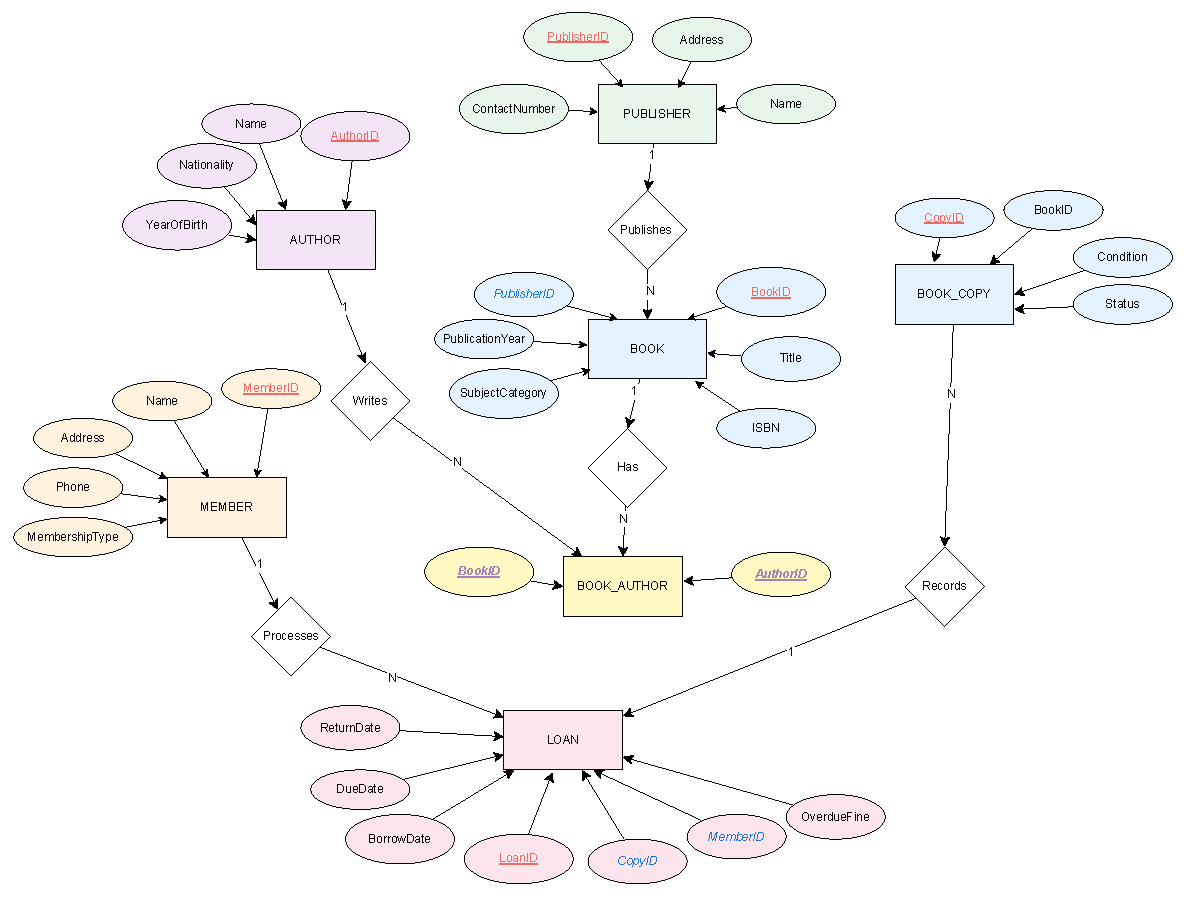
\includegraphics[width=\textwidth]{images/Library_Management_ERD_hinhthoi.drawio.pdf}
\caption{Sơ đồ Thực thể - Mối quan hệ (ERD) cho hệ thống Quản lý Thư viện}
\label{fig:erd}
\end{figure}
% \end{landscape} % Kết thúc xoay ngang, trang sau sẽ tự về dọc lại

\textbf{Chú thích ký hiệu trong sơ đồ:}
\begin{itemize}
\item Khóa chính (Primary Key - PK): Được viết bằng chữ màu đỏ và gạch chân (Ví dụ: BookID, AuthorID, LoanID).
\item Khóa ngoại (Foreign Key - FK): Được viết bằng chữ màu xanh dương và in nghiêng (Ví dụ: PublisherID trong bảng BOOK, MemberID trong bảng LOAN).
\item Khóa chính vừa là Khóa ngoại (PK, FK): -Được viết bằng chữ màu tím, vừa gạch chân vừa in nghiêng.
\end{itemize}


\subsubsection{Mô tả chi tiết các mối quan hệ}

\textbf{1. Publishes (1:N) - PUBLISHER đến BOOK}
\begin{itemize}
    \item Một nhà xuất bản có thể xuất bản nhiều cuốn sách
    \item Mỗi cuốn sách được xuất bản bởi đúng một nhà xuất bản
    \item Ràng buộc: \attr{PublisherID} trong \entity{BOOK} là khóa ngoại tham chiếu đến \entity{PUBLISHER}
\end{itemize}

\textbf{2. Writes (M:N) - AUTHOR đến BOOK}
\begin{itemize}
    \item Một tác giả có thể viết nhiều cuốn sách
    \item Một cuốn sách có thể có nhiều tác giả
    \item Cần bảng trung gian \entity{BOOK\_AUTHOR} để quản lý mối quan hệ này
    \item Bảng \entity{BOOK\_AUTHOR} có khóa chính kép (\attr{BookID}, \attr{AuthorID})
\end{itemize}

\textbf{3. Has (1:N) - BOOK đến BOOK\_COPY}
\begin{itemize}
    \item Một cuốn sách (title) có thể có nhiều bản sao vật lý
    \item Mỗi bản sao thuộc về một cuốn sách duy nhất
    \item Ràng buộc: \attr{BookID} trong \entity{BOOK\_COPY} là khóa ngoại tham chiếu đến \entity{BOOK}
    \item Khi xóa sách, tất cả bản sao cũng bị xóa (ON DELETE CASCADE)
\end{itemize}

\textbf{4. Processes (1:N) - MEMBER đến LOAN}
\begin{itemize}
    \item Một thành viên có thể tạo nhiều giao dịch mượn
    \item Mỗi giao dịch mượn thuộc về một thành viên
    \item Ràng buộc: \attr{MemberID} trong \entity{LOAN} là khóa ngoại tham chiếu đến \entity{MEMBER}
    \item Lưu trữ lịch sử đầy đủ của các giao dịch mượn/trả
\end{itemize}

\textbf{5. Records (1:1) - LOAN đến BOOK\_COPY}
\begin{itemize}
    \item Một giao dịch mượn ghi nhận một bản sao sách cụ thể
    \item Mỗi bản sao tại một thời điểm chỉ được ghi nhận trong một giao dịch đang hoạt động
    \item Ràng buộc: \attr{CopyID} trong \entity{LOAN} là khóa ngoại tham chiếu đến \entity{BOOK\_COPY}
    \item Không thể có hai giao dịch mượn đang hoạt động cho cùng một bản sao
\end{itemize}

\textbf{Lưu ý về thiết kế:}
\begin{itemize}
    \item Thành viên không trực tiếp kết nối đến bản sao sách
    \item Việc mượn sách được thực hiện thông qua thực thể \entity{LOAN}
    \item Thiết kế này cho phép lưu trữ đầy đủ thông tin về mỗi lần mượn: ngày mượn, ngày hết hạn, ngày trả, và phí phạt
    \item Hỗ trợ truy vấn lịch sử mượn của thành viên và thống kê báo cáo
\end{itemize}

\subsubsection{Các quyết định thiết kế chính}

\textbf{1. Tách BOOK và BOOK\_COPY:}
\begin{itemize}
    \item \entity{BOOK} lưu thông tin chung về title/ISBN
    \item \entity{BOOK\_COPY} lưu thông tin về từng bản sao vật lý
    \item Giúp quản lý chính xác số lượng sách có sẵn
\end{itemize}

\textbf{2. Sử dụng bảng trung gian BOOK\_AUTHOR:}
\begin{itemize}
    \item Hỗ trợ mối quan hệ M:N giữa \entity{AUTHOR} và \entity{BOOK}
    \item Cho phép một sách có nhiều tác giả
    \item Cho phép một tác giả có nhiều sách
\end{itemize}

\textbf{3. Tách LOAN thành thực thể riêng:}
\begin{itemize}
    \item Lưu trữ đầy đủ thông tin về mỗi giao dịch mượn
    \item Hỗ trợ tính toán phí phạt
    \item Lưu trữ lịch sử mượn/trả đầy đủ
\end{itemize}

\subsection{Kết luận báo cáo 1}

\subsubsection{Tổng kết kết quả}

Báo cáo 1 đã hoàn thành phân tích và thiết kế sơ đồ ERD cho hệ thống quản lý thư viện:

\textbf{1. Xác định được 6 thực thể chính:}
\begin{itemize}
    \item \entity{BOOK} - 6 thuộc tính
    \item \entity{AUTHOR} - 4 thuộc tính
    \item \entity{PUBLISHER} - 4 thuộc tính
    \item \entity{BOOK\_COPY} - 4 thuộc tính
    \item \entity{MEMBER} - 5 thuộc tính
    \item \entity{LOAN} - 7 thuộc tính
\end{itemize}

\textbf{2. Xác định được 5 mối quan hệ:}
\begin{itemize}
    \item Publishes (1:N) - \entity{PUBLISHER} → \entity{BOOK}
    \item Writes (M:N) - \entity{AUTHOR} ↔ \entity{BOOK} (qua \entity{BOOK\_AUTHOR})
    \item Has (1:N) - \entity{BOOK} → \entity{BOOK\_COPY}
    \item Processes (1:N) - \entity{MEMBER} → \entity{LOAN}
    \item Records (1:1) - \entity{LOAN} → \entity{BOOK\_COPY}
\end{itemize}

\textbf{Lưu ý về thiết kế quan hệ:}
\begin{itemize}
    \item Việc mượn sách được mô hình hóa thông qua thực thể \entity{LOAN}, không phải quan hệ trực tiếp giữa \entity{MEMBER} và \entity{BOOK\_COPY}
    \item Thành viên tạo giao dịch \entity{LOAN}, và giao dịch đó ghi nhận bản sao sách được mượn
    \item Thiết kế này cho phép lưu trữ đầy đủ thông tin về mỗi lần mượn và theo dõi lịch sử
\end{itemize}

\textbf{3. Xác định được 1 bảng trung gian:}
\begin{itemize}
    \item \entity{BOOK\_AUTHOR} - quản lý mối quan hệ nhiều-nhiều
\end{itemize}

\subsubsection{Chuẩn bị cho báo cáo 2}

Báo cáo 2 sẽ chuyển đổi sơ đồ ERD sang mô hình quan hệ (Relational Data Model) và thực hiện:
\begin{enumerate}
    \item Chuyển đổi thực thể thành bảng (tables)
    \item Xác định khóa chính và khóa ngoại
    \item Xác định các lược đồ quan hệ (relation schemas)
    \item Nhận dạng các mẫu không chuẩn hóa
    \item Chuẩn bị cho quá trình chuẩn hóa trong báo cáo 3
\end{enumerate}

\subsubsection{Đánh giá chất lượng thiết kế}

\begin{itemize}
    \item \textbf{Tính đầy đủ:} Tất cả các thực thể và mối quan hệ cần thiết đã được xác định
    \item \textbf{Tính chính xác:} Bội số và các ràng buộc được xác định đúng theo yêu cầu
    \item \textbf{Tính rõ ràng:} Sơ đồ ERD thể hiện rõ cấu trúc dữ liệu
    \item \textbf{Khả năng mở rộng:} Thiết kế cho phép thêm các thực thể mới trong tương lai
\end{itemize}

%===========================================================
% SECTION 2: REPORT 2 - RELATIONAL MODEL DESIGN
%===========================================================
\newpage
\section{BÁO CÁO 2: MÔ HÌNH QUAN HỆ (RELATIONAL DATA MODEL)}

\subsection{Giới thiệu báo cáo 2}

Báo cáo 2 là bước tiếp theo trong quá trình thiết kế cơ sở dữ liệu, chuyển đổi từ sơ đồ Thực thể - Mối quan hệ (ERD) đã hoàn thiện trong Báo cáo 1 sang \textbf{Mô hình Quan hệ (Relational Data Model)}. Đây là bước quan trọng để chuẩn bị cho quá trình chuẩn hóa dữ liệu trong Báo cáo 3.

\textbf{Mục tiêu của Báo cáo 2:}
\begin{itemize}
    \item Chuyển đổi các thực thể (entities) thành các bảng (tables/relation schemas)
    \item Xác định khóa chính (Primary Keys) và khóa ngoại (Foreign Keys)
    \item Thiết lập các mối quan hệ giữa các bảng thông qua khóa ngoại
    \item Xác định các phụ thuộc hàm (Functional Dependencies)
    \item Nhận dạng các mẫu chưa chuẩn hóa để chuẩn bị cho chuẩn hóa 3NF
\end{itemize}

\subsection{Cơ sở lý thuyết}

\subsubsection{Mô hình Quan hệ (Relational Model)}

\textbf{Định nghĩa:} Mô hình quan hệ là một mô hình cơ sở dữ liệu thể hiện dữ liệu dưới dạng các quan hệ (relations), mà người dùng có thể nhận thức dưới dạng các bảng (tables) gồm các hàng (rows) và cột (columns).

\textbf{Các thành phần cơ bản:}

\begin{table}[H]
\centering
\caption{Thành phần của Mô hình Quan hệ}
\begin{tabular}{@{}|l|p{9cm}|@{}}
\hline
\textbf{Thành phần} & \textbf{Mô tả} \\ \hline
\textbf{Relation (Quan hệ)} & Một bảng 2D chứa dữ liệu, tương ứng với một thực thể trong ERD \\ \hline
\textbf{Tuple (Bộ)} & Một hàng trong bảng, tương ứng với một bản ghi hoặc một thể hiện của thực thể \\ \hline
\textbf{Attribute (Thuộc tính)} & Một cột trong bảng, tương ứng với một thuộc tính của thực thể \\ \hline
\textbf{Domain (Miền giá trị)} & Tập hợp các giá trị hợp lệ cho một thuộc tính \\ \hline
\textbf{Degree (Bậc)} & Số lượng thuộc tính trong một quan hệ \\ \hline
\textbf{Cardinality (Độ)} & Số lượng bộ trong một quan hệ \\ \hline
\end{tabular}
\end{table}

\subsubsection{Khóa chính (Primary Key)}

\textbf{Định nghĩa:} Khóa chính là một thuộc tính hoặc tập hợp các thuộc tính định danh duy nhất mỗi bộ trong một quan hệ.

\textbf{Đặc điểm:}
\begin{itemize}
    \item \textbf{Tính duy nhất:} Không có hai bộ nào có cùng giá trị khóa chính
    \item \textbf{Tính không rỗng:} Khóa chính không thể chứa giá trị NULL
    \item \textbf{Tính ổn định:} Giá trị khóa chính không nên thay đổi
\end{itemize}

\textbf{Ký hiệu:} Gạch dưới thuộc tính (ví dụ: \underline{BookID}) hoặc ký hiệu PK

\subsubsection{Khóa ngoại (Foreign Key)}

\textbf{Định nghĩa:} Khóa ngoại là một thuộc tính trong một quan hệ tham chiếu đến khóa chính của một quan hệ khác, thiết lập mối quan hệ giữa hai bảng.

\textbf{Đặc điểm:}
\begin{itemize}
    \item \textbf{Tham chiếu:} Giá trị khóa ngoại phải khớp với giá trị khóa chính được tham chiếu, hoặc là NULL
    \item \textbf{Tính toàn vẹn:} Đảm bảo tính toàn vẹn tham chiếu (Referential Integrity)
    \item \textbf{Hành vi cascade:} Xác định điều gì xảy ra khi dữ liệu được tham chiếu bị xóa hoặc cập nhật
\end{itemize}

\textbf{Ký hiệu:} Chỉ mũi tên từ khóa ngoại sang khóa chính được tham chiếu

\subsubsection{Phụ thuộc hàm (Functional Dependency)}

\textbf{Định nghĩa:} Phụ thuộc hàm là một ràng buộc giữa hai tập hợp thuộc tính trong một quan hệ. Được ký hiệu là $X \rightarrow Y$, đọc là "X xác định Y" hoặc "Y phụ thuộc hàm vào X".

\textbf{Định nghĩa toán học:} Trong một quan hệ R, $X \rightarrow Y$ nếu và chỉ nếu mỗi giá trị của X liên kết với chính xác một giá trị của Y.

\textbf{Ví dụ:}
\begin{itemize}
    \item \texttt{BookID} $\rightarrow$ \texttt{Title}: Mã sách xác định tên sách
    \item \texttt{BookID} $\rightarrow$ \texttt{ISBN, PublicationYear, PublisherID}
    \item \texttt{MemberID} $\rightarrow$ \texttt{Name, Address, Phone}
\end{itemize}

\subsection{Quy tắc chuyển đổi từ ERD sang Mô hình Quan hệ}

\subsubsection{Quy tắc cơ bản}

\begin{table}[H]
\centering
\caption{Quy tắc chuyển đổi ERD sang Relational Model}
\begin{tabular}{@{}|l|p{9cm}|@{}}
\hline
\textbf{Thành phần ERD} & \textbf{Quy tắc chuyển đổi} \\ \hline
\textbf{Thực thể mạnh} & Chuyển thành một bảng (table) riêng biệt \\ \hline
\textbf{Thuộc tính} & Chuyển thành cột (column) của bảng \\ \hline
\textbf{Khóa chính} & Chuyển thành PRIMARY KEY constraint \\ \hline
\textbf{Quan hệ 1:1} & Thêm khóa ngoại vào một trong hai bảng, thường là bảng có tham gia bắt buộc \\ \hline
\textbf{Quan hệ 1:N} & Thêm khóa ngoại vào bảng "N" (bên nhiều) tham chiếu đến bảng "1" (bên một) \\ \hline
\textbf{Quan hệ M:N} & Tạo bảng trung gian (junction table) với hai khóa ngoại \\ \hline
\textbf{Thực thể yếu} & Thêm khóa ngoại tham chiếu đến thực thể sở hữu, có thể tạo khóa chính kép \\ \hline
\end{tabular}
\end{table}

\subsubsection{Quy tắc chi tiết cho từng loại quan hệ}

\textbf{1. Quan hệ Một-Nhiều (1:N):}

\begin{itemize}
    \item Bên "1": Thực thể có khóa chính PK
    \item Bên "N": Thêm thuộc tính khóa ngoại FK tham chiếu đến PK của bên "1"
    \item \textbf{Ví dụ:} \entity{PUBLISHER} (1) $\rightarrow$ \entity{BOOK} (N)
    \item \entity{BOOK} có \attr{PublisherID} là khóa ngoại tham chiếu đến \entity{PUBLISHER}
\end{itemize}

\textbf{2. Quan hệ Nhiều-Nhiều (M:N):}

\begin{itemize}
    \item Tạo bảng trung gian mới
    \item Bảng trung gian có hai khóa ngoại FK tham chiếu đến PK của hai thực thể
    \item Khóa chính của bảng trung gian là kết hợp của hai khóa ngoại
    \item \textbf{Ví dụ:} \entity{AUTHOR} (M) $\leftrightarrow$ \entity{BOOK} (N)
    \item Tạo \entity{BOOK\_AUTHOR} với PK (\attr{BookID}, \attr{AuthorID})
\end{itemize}

\textbf{3. Quan hệ Một-Một (1:1):}

\begin{itemize}
    \item Thêm khóa ngoại vào một trong hai bảng
    \item Khóa ngoại vừa là khóa ngoại vừa là khóa chính
    \item \textbf{Ví dụ:} \entity{LOAN} (1) $\leftrightarrow$ \entity{BOOK\_COPY} (1)
    \item \entity{LOAN} có \attr{CopyID} là FK và tham chiếu độc nhất
\end{itemize}

\subsection{Chuyển đổi ERD sang Lược đồ Quan hệ}

\subsubsection{Lược đồ quan hệ cho các thực thể cơ bản}

\textbf{1. PUBLISHER (Nhà xuất bản)}

$$
\texttt{PUBLISHER}(\underline{\texttt{PublisherID}}, \texttt{Name}, \texttt{Address}, \texttt{ContactNumber})
$$

\begin{table}[H]
\centering
\caption{Lược đồ quan hệ PUBLISHER}
\begin{tabular}{@{}|l|l|l|l|@{}}
\hline
\textbf{Tên bảng} & \textbf{Khóa chính} & \textbf{Thuộc tính} & \textbf{Kiểu dữ liệu} \\ \hline
\multirow{4}{*}{\texttt{PUBLISHER}} & \multirow{4}{*}{\underline{\texttt{PublisherID}}} & \texttt{PublisherID} & INT \\ \cline{3-4}
& & \texttt{Name} & VARCHAR(255) \\ \cline{3-4}
& & \texttt{Address} & VARCHAR(500) \\ \cline{3-4}
& & \texttt{ContactNumber} & VARCHAR(50) \\ \hline
\end{tabular}
\end{table}

\textbf{2. AUTHOR (Tác giả)}

$$
\texttt{AUTHOR}(\underline{\texttt{AuthorID}}, \texttt{Name}, \texttt{Nationality}, \texttt{YearOfBirth})
$$

\begin{table}[H]
\centering
\caption{Lược đồ quan hệ AUTHOR}
\begin{tabular}{@{}|l|l|l|l|@{}}
\hline
\textbf{Tên bảng} & \textbf{Khóa chính} & \textbf{Thuộc tính} & \textbf{Kiểu dữ liệu} \\ \hline
\multirow{4}{*}{\texttt{AUTHOR}} & \multirow{4}{*}{\underline{\texttt{AuthorID}}} & \texttt{AuthorID} & INT \\ \cline{3-4}
& & \texttt{Name} & VARCHAR(255) \\ \cline{3-4}
& & \texttt{Nationality} & VARCHAR(100) \\ \cline{3-4}
& & \texttt{YearOfBirth} & INT \\ \hline
\end{tabular}
\end{table}

\textbf{3. MEMBER (Thành viên)}

$$
\texttt{MEMBER}(\underline{\texttt{MemberID}}, \texttt{Name}, \texttt{Address}, \texttt{Phone}, \texttt{MembershipType})
$$

\begin{table}[H]
\centering
\caption{Lược đồ quan hệ MEMBER}
\begin{tabular}{@{}|l|l|l|l|@{}}
\hline
\textbf{Tên bảng} & \textbf{Khóa chính} & \textbf{Thuộc tính} & \textbf{Kiểu dữ liệu} \\ \hline
\multirow{5}{*}{\texttt{MEMBER}} & \multirow{5}{*}{\underline{\texttt{MemberID}}} & \texttt{MemberID} & INT \\ \cline{3-4}
& & \texttt{Name} & VARCHAR(255) \\ \cline{3-4}
& & \texttt{Address} & VARCHAR(500) \\ \cline{3-4}
& & \texttt{Phone} & VARCHAR(20) \\ \cline{3-4}
& & \texttt{MembershipType} & VARCHAR(50) \\ \hline
\end{tabular}
\end{table}

\textbf{4. BOOK (Sách)}

$$
\texttt{BOOK}(\underline{\texttt{BookID}}, \texttt{ISBN}, \texttt{Title}, \texttt{SubjectCategory}, \texttt{PublicationYear}, \texttt{PublisherID})
$$

\begin{table}[H]
\centering
\caption{Lược đồ quan hệ BOOK}
\begin{tblr}{
  colspec = {|c|c|c|l|l|}, % Định dạng cột: Giữa | Giữa | Giữa | Trái | Trái
  vlines, hlines,          % Kẻ khung
  rows = {m},              % Căn giữa dọc tất cả các hàng
  row{1} = {font=\bfseries, c}, % Dòng tiêu đề: In đậm, căn giữa
  cell{2}{1} = {r=6}{c},   % Ô BOOK: Gộp 6 hàng, căn giữa
  cell{2}{2} = {r=6}{c},   % Ô BookID: Gộp 6 hàng, căn giữa
  cell{2}{3} = {r=6}{c},        % Ô PublisherID: Gộp 6 hàng, căn giữa
}
Tên bảng & Khóa chính & Khóa ngoại & Thuộc tính & Kiểu dữ liệu \\
BOOK     & \underline{BookID} & PublisherID & BookID           & INT \\
         &            &            & ISBN             & VARCHAR(17) \\
         &            &            & Title            & VARCHAR(255) \\
         &            &            & SubjectCategory  & VARCHAR(100) \\
         &            &            & PublicationYear  & INT \\
         &            &            & PublisherID      & INT \\
\end{tblr}
\end{table}

\textbf{Ghi chú:}
\begin{itemize}
    \item \texttt{PublisherID} là khóa ngoại tham chiếu đến \texttt{PUBLISHER(PublisherID)}
    \item Ký hiệu: $\texttt{BOOK.PublisherID} \rightarrow \texttt{PUBLISHER.PublisherID}$
\end{itemize}

\textbf{5. BOOK\_COPY (Bản sao sách)}

$$
\texttt{BOOK\_COPY}(\underline{\texttt{CopyID}}, \texttt{BookID}, \texttt{Condition}, \texttt{Status})
$$

\begin{table}[H]
\centering
\caption{Lược đồ quan hệ BOOK\_COPY}
\begin{tblr}{
  colspec = {|c|c|c|l|l|}, 
  vlines, hlines,
  rows = {m},
  row{1} = {font=\bfseries, c},
  cell{2}{1} = {r=4}{c}, % Gộp 4 hàng cho tên bảng
  cell{2}{2} = {r=4}{c}, % Gộp 4 hàng cho khóa chính
  cell{2}{3} = {r=4}{c}, % Gộp 4 hàng cho khóa ngoại
}
Tên bảng & Khóa chính & Khóa ngoại & Thuộc tính & Kiểu dữ liệu \\
BOOK\_COPY & \underline{CopyID} & BookID & CopyID & INT \\
           &           &        & BookID & INT \\
           &           &        & Condition & VARCHAR(50) \\
           &           &        & Status    & VARCHAR(20) \\
\end{tblr}
\end{table}

\textbf{Ghi chú:}
\begin{itemize}
    \item \texttt{BookID} là khóa ngoại tham chiếu đến \texttt{BOOK(BookID)}
    \item Đây là thực thể yếu (weak entity) phụ thuộc vào \texttt{BOOK}
    \item Ký hiệu: $\texttt{BOOK\_COPY.BookID} \rightarrow \texttt{BOOK.BookID}$
\end{itemize}

\textbf{6. LOAN (Mượn/trả)}

$$
\texttt{LOAN}(\underline{\texttt{LoanID}}, \texttt{MemberID}, \texttt{CopyID}, \texttt{BorrowDate}, \texttt{DueDate}, \texttt{ReturnDate}, \texttt{OverdueFine})
$$

\begin{table}[H]
\centering
\caption{Lược đồ quan hệ LOAN}
\begin{tblr}{
  colspec = {|c|c|c|l|l|}, % 5 cột: Giữa, Giữa, Giữa, Trái, Trái
  vlines, hlines,
  rows = {m},            % Căn giữa dọc cho tất cả các ô
  row{1} = {font=\bfseries, c}, % Dòng đầu in đậm và căn giữa ngang
  cell{2}{1} = {r=7}{c}, % Gộp 7 hàng cho tên bảng LOAN
  cell{2}{2} = {r=7}{c}, % Gộp 7 hàng cho khóa chính LoanID
  cell{2}{3} = {r=7}{c}, % Gộp 7 hàng cho các khóa ngoại
}
Tên bảng & Khóa chính & Khóa ngoại & Thuộc tính & Kiểu dữ liệu \\
LOAN     & \underline{LoanID} & {MemberID, \\ CopyID} & LoanID & INT \\
         &            &            & MemberID     & INT \\
         &            &            & CopyID       & INT \\
         &            &            & BorrowDate   & DATE \\
         &            &            & DueDate      & DATE \\
         &            &            & ReturnDate   & DATE \\
         &            &            & OverdueFine  & DECIMAL(10,2) \\
\end{tblr}
\end{table}

\textbf{Ghi chú:}
\begin{itemize}
    \item \texttt{MemberID} là khóa ngoại tham chiếu đến \texttt{MEMBER(MemberID)}
    \item \texttt{CopyID} là khóa ngoại tham chiếu đến \texttt{BOOK\_COPY(CopyID)}
    \item Ký hiệu:
    \begin{itemize}
        \item $\texttt{LOAN.MemberID} \rightarrow \texttt{MEMBER.MemberID}$
        \item $\texttt{LOAN.CopyID} \rightarrow \texttt{BOOK\_COPY.CopyID}$
    \end{itemize}
\end{itemize}

\subsubsection{Bảng trung gian cho quan hệ M:N}

\textbf{BOOK\_AUTHOR (Bảng trung gian Sách-Tác giả)}

$$
\texttt{BOOK\_AUTHOR}(\underline{\texttt{BookID}}, \underline{\texttt{AuthorID}})
$$

\begin{table}[H]
\centering
\caption{Lược đồ quan hệ BOOK\_AUTHOR (Bảng trung gian)}
\begin{tblr}{
  colspec = {|c|c|X[l]|X[l]|}, % Cột X sẽ tự động co giãn để vừa khít trang giấy
  vlines, hlines,
  rows = {m},                 % Căn giữa dọc
  row{1} = {font=\bfseries, c}, % Dòng tiêu đề in đậm, căn giữa ngang
  cell{2}{1} = {r=2}{c},      % Gộp 2 hàng cho tên bảng
  cell{2}{2} = {r=2}{c},      % Gộp 2 hàng cho khóa chính kép
}
Tên bảng & Khóa chính & Khóa ngoại & Mô tả \\
BOOK\_AUTHOR & \underline{BookID}, \underline{AuthorID} & BookID $\rightarrow$ BOOK (BookID) & Khóa ngoại đến BOOK \\
             &                                          & AuthorID $\rightarrow$ AUTHOR (AuthorID) & Khóa ngoại đến AUTHOR \\
\end{tblr}
\end{table}

\textbf{Ghi chú:}
\begin{itemize}
    \item \textbf{Khóa chính kép:} (\texttt{BookID}, \texttt{AuthorID})
    \item Mỗi cặp (BookID, AuthorID) là duy nhất - một tác giả chỉ được liệt kê một lần cho mỗi sách
    \item Quan hệ này thể hiện mối quan hệ nhiều-nhiều giữa \texttt{AUTHOR} và \texttt{BOOK}
\end{itemize}

\subsection{Tổng hợp Lược đồ Quan hệ Hệ Thống}

\subsubsection{Tất cả Lược đồ Quan hệ}

\textbf{Tóm tắt tất cả 7 bảng trong hệ thống:}

\begin{table}[H]
\centering
\renewcommand{\arraystretch}{1.5} % Giúp các dòng giãn cách thoáng hơn
\begin{tabular}{l p{12cm}}
\textbf{PUBLISHER} & (\underline{PublisherID}, Name, Address, ContactNumber) \\
\textbf{AUTHOR}    & (\underline{AuthorID}, Name, Nationality, YearOfBirth) \\
\textbf{MEMBER}    & (\underline{MemberID}, Name, Address, Phone, MembershipType) \\
\textbf{BOOK}      & (\underline{BookID}, ISBN, Title, SubjectCategory, PublicationYear, PublisherID$^*$) \\
\textbf{BOOK\_COPY} & (\underline{CopyID}, BookID$^\dagger$, Condition, Status) \\
\textbf{LOAN}      & (\underline{LoanID}, MemberID$^\ddagger$, CopyID$^\ddagger$, BorrowDate, DueDate, ReturnDate, OverdueFine) \\
\textbf{BOOK\_AUTHOR} & (\underline{BookID}$^\dagger$, \underline{AuthorID}$^\ddagger$) \\
\end{tabular}
\end{table}

\vspace{0.3cm}
\noindent \textbf{Chú thích:}
\begin{itemize}[leftmargin=1.5cm, labelsep=0.3cm, itemsep=0pt]
    \item[$^*, \dagger, \ddagger$] Các ký hiệu phía sau tên thuộc tính chỉ \textbf{Khóa ngoại} (Foreign Key) tham chiếu đến bảng tương ứng.
    \item[\underline{\hspace{0.3cm}}] Các thuộc tính được gạch chân đóng vai trò là \textbf{Khóa chính} (Primary Key).
\end{itemize}

\begin{table}[H]
\centering
\caption{Tổng hợp các bảng và khóa}
\begin{tblr}{
  colspec = {|c|l|l|X[l]|}, % Cột cuối tự động giãn rộng
  vlines, hlines,
  rows = {m},                 % Căn giữa dọc cho tất cả các hàng
  row{1} = {font=\bfseries, c}, % Dòng tiêu đề: In đậm, căn giữa ngang
  cell{7}{1,2,3} = {r=2}{l},    % Gộp hàng cho bảng LOAN
  cell{9}{1,2,3} = {r=2}{l},    % Gộp hàng cho bảng BOOK_AUTHOR
}
STT & Tên bảng & Khóa chính (PK) & Khóa ngoại (FK) \\
1 & PUBLISHER   & PublisherID & -- \\
2 & AUTHOR      & AuthorID    & -- \\
3 & MEMBER      & MemberID    & -- \\
4 & BOOK        & BookID      & PublisherID $\rightarrow$ PUBLISHER \\
5 & BOOK\_COPY  & CopyID      & BookID $\rightarrow$ BOOK \\
6 & LOAN        & LoanID      & MemberID $\rightarrow$ MEMBER \\
  &             &             & CopyID $\rightarrow$ BOOK\_COPY \\
7 & BOOK\_AUTHOR & BookID, AuthorID & BookID $\rightarrow$ BOOK \\
  &             &                   & AuthorID $\rightarrow$ AUTHOR \\
\end{tblr}
\end{table}

\subsubsection{Sơ đồ Mô hình Quan hệ (Relational Data Model Diagram)}

% TODO: Insert your RDM diagram here
% Replace the filename below with your actual diagram file
\begin{figure}[H]
\centering
\includegraphics[width=\textwidth,keepaspectratio]{images/RDM_Library_Management.pdf}
% \includegraphics[width=\textwidth,keepaspectratio]{images/RDM_Library_Management.png}
\caption{Sơ đồ Mô hình Quan hệ (Relational Data Model) cho hệ thống Quản lý Thư viện}
\label{fig:rdm}
\end{figure}

\textbf{Ghi chú ký hiệu trong sơ đồ:}
\begin{itemize}
\item \textbf{PK (Primary Key):} Khóa chính - được hiển thị ở đầu danh sách cột
\item \textbf{FK (Foreign Key):} Khóa ngoại - tham chiếu đến bảng khác
\item \textbf{Đường nối:} Thể hiện mối quan hệ giữa các bảng
\end{itemize}

\subsection{Phụ thuộc Hàm (Functional Dependencies)}

\subsubsection{Định nghĩa và Ký hiệu}

\textbf{Phụ thuộc hàm (Functional Dependency - FD)} mô tả mối quan hệ giữa các thuộc tính trong một bảng. Nếu thuộc tính X xác định thuộc tính Y, ta ký hiệu: $X \rightarrow Y$

\textbf{Ví dụ:} Nếu biết mã sách ($\texttt{BookID}$), ta biết được tên sách ($\texttt{Title}$), ISBN, năm xuất bản, và mã nhà xuất bản. Ký hiệu:
$$ \texttt{BookID} \rightarrow \texttt{Title, ISBN, PublicationYear, PublisherID} $$

\subsubsection{Các Phụ thuộc Hàm cho từng Bảng}

\textbf{1. Bảng PUBLISHER:}

$$
\begin{aligned}
\texttt{PublisherID} &\rightarrow \texttt{Name} \\
\texttt{PublisherID} &\rightarrow \texttt{Address} \\
\texttt{PublisherID} &\rightarrow \texttt{ContactNumber}
\end{aligned}
$$

\textbf{Gộp:} $\texttt{PublisherID} \rightarrow \texttt{Name, Address, ContactNumber}$

\textbf{Giải thích:} Mã nhà xuất bản xác định duy nhất tên, địa chỉ và số điện thoại liên hệ của nhà xuất bản đó.

\vspace{0.5cm}

\textbf{2. Bảng AUTHOR:}

$$
\begin{aligned}
\texttt{AuthorID} &\rightarrow \texttt{Name} \\
\texttt{AuthorID} &\rightarrow \texttt{Nationality} \\
\texttt{AuthorID} &\rightarrow \texttt{YearOfBirth}
\end{aligned}
$$

\textbf{Gộp:} $\texttt{AuthorID} \rightarrow \texttt{Name, Nationality, YearOfBirth}$

\textbf{Giải thích:} Mã tác giả xác định duy nhất tên, quốc tịch và năm sinh của tác giả đó.

\vspace{0.5cm}

\textbf{3. Bảng MEMBER:}

$$
\begin{aligned}
\texttt{MemberID} &\rightarrow \texttt{Name} \\
\texttt{MemberID} &\rightarrow \texttt{Address} \\
\texttt{MemberID} &\rightarrow \texttt{Phone} \\
\texttt{MemberID} &\rightarrow \texttt{MembershipType}
\end{aligned}
$$

\textbf{Gộp:} $\texttt{MemberID} \rightarrow \texttt{Name, Address, Phone, MembershipType}$

\textbf{Giải thích:} Mã thành viên xác định duy nhất tên, địa chỉ, số điện thoại và loại thành viên.

\vspace{0.5cm}

\textbf{4. Bảng BOOK:}

$$
\begin{aligned}
\texttt{BookID} &\rightarrow \texttt{ISBN} \\
\texttt{BookID} &\rightarrow \texttt{Title} \\
\texttt{BookID} &\rightarrow \texttt{SubjectCategory} \\
\texttt{BookID} &\rightarrow \texttt{PublicationYear} \\
\texttt{BookID} &\rightarrow \texttt{PublisherID}
\end{aligned}
$$

\textbf{Gộp:} $\texttt{BookID} \rightarrow \texttt{ISBN, Title, SubjectCategory, PublicationYear, PublisherID}$

\textbf{Giải thích:} Mã sách xác định duy nhất ISBN, tên, thể loại, năm xuất bản và mã nhà xuất bản của sách đó.

\vspace{0.5cm}

\textbf{5. Bảng BOOK\_COPY:}

$$
\begin{aligned}
\texttt{CopyID} &\rightarrow \texttt{BookID} \\
\texttt{CopyID} &\rightarrow \texttt{Condition} \\
\texttt{CopyID} &\rightarrow \texttt{Status}
\end{aligned}
$$

\textbf{Gộp:} $\texttt{CopyID} \rightarrow \texttt{BookID, Condition, Status}$

\textbf{Giải thích:} Mã bản sao xác định duy nhất mã sách mà bản sao thuộc về, tình trạng và trạng thái hiện tại của bản sao.

\vspace{0.5cm}

\textbf{6. Bảng LOAN:}

$$
\begin{aligned}
\texttt{LoanID} &\rightarrow \texttt{MemberID} \\
\texttt{LoanID} &\rightarrow \texttt{CopyID} \\
\texttt{LoanID} &\rightarrow \texttt{BorrowDate} \\
\texttt{LoanID} &\rightarrow \texttt{DueDate} \\
\texttt{LoanID} &\rightarrow \texttt{ReturnDate} \\
\texttt{LoanID} &\rightarrow \texttt{OverdueFine}
\end{aligned}
$$

\textbf{Gộp:} $\texttt{LoanID} \rightarrow \texttt{MemberID, CopyID, BorrowDate, DueDate, ReturnDate, OverdueFine}$

\textbf{Giải thích:} Mã giao dịch mượn xác định duy nhất thành viên mượn, bản sao được mượn, ngày mượn, ngày hết hạn, ngày trả và phí phạt.

\vspace{0.5cm}

\textbf{7. Bảng BOOK\_AUTHOR (Bảng trung gian):}

Bảng này có khóa chính kép ($\texttt{BookID}, \texttt{AuthorID}$), nên không có phụ thuộc hàm từ một thuộc tính đơn lẻ. Các phụ thuộc hàm được xác định bởi cả hai khóa chính:

$$
\begin{aligned}
\texttt{BookID, AuthorID} &\rightarrow \texttt{BookID} \\
\texttt{BookID, AuthorID} &\rightarrow \texttt{AuthorID}
\end{aligned}
$$

\textbf{Giải thích:} Cả hai thuộc tính đều là một phần của khóa chính, không có phụ thuộc hàm từ khóa này sang khóa kia.

\subsubsection{Tổng hợp các Phụ thuộc Hàm}

\begin{table}[H]
\centering
\caption{Tổng hợp Phụ thuộc Hàm cho tất cả các bảng}
\begin{tabular}{@{}|l|p{10cm}|@{}}
\hline
\textbf{Bảng} & \textbf{Phụ thuộc Hàm} \\ \hline
\texttt{PUBLISHER} & $\texttt{PublisherID} \rightarrow \texttt{Name, Address, ContactNumber}$ \\ \hline
\texttt{AUTHOR} & $\texttt{AuthorID} \rightarrow \texttt{Name, Nationality, YearOfBirth}$ \\ \hline
\texttt{MEMBER} & $\texttt{MemberID} \rightarrow \texttt{Name, Address, Phone, MembershipType}$ \\ \hline
\texttt{BOOK} & $\texttt{BookID} \rightarrow \texttt{ISBN, Title, SubjectCategory, PublicationYear, PublisherID}$ \\ \hline
\texttt{BOOK\_COPY} & $\texttt{CopyID} \rightarrow \texttt{BookID, Condition, Status}$ \\ \hline
\texttt{LOAN} & $\texttt{LoanID} \rightarrow \texttt{MemberID, CopyID, BorrowDate, DueDate, ReturnDate, OverdueFine}$ \\ \hline
\texttt{BOOK\_AUTHOR} & $\texttt{(BookID, AuthorID)} \rightarrow \texttt{BookID, AuthorID}$ (khóa chính kép) \\ \hline
\end{tabular}
\end{table}

\subsection{Đánh giá Mô hình Quan hệ}

\subsubsection{Tính toàn vẹn dữ liệu (Data Integrity)}

\textbf{1. Toàn vẹn thực thể (Entity Integrity):}
\begin{itemize}
    \item Mỗi bảng có khóa chính (Primary Key) xác định duy nhất mỗi dòng
    \item Khóa chính không chứa giá trị NULL
    \item Đảm bảo không có các bản ghi trùng lặp
\end{itemize}

\textbf{2. Toàn vẹn tham chiếu (Referential Integrity):}
\begin{itemize}
    \item Mọi khóa ngoại đều tham chiếu đến khóa chính hợp lệ của bảng khác
    \item Không thể có giá trị khóa ngoại "mồ côi" (orphaned records)
    \item Được thực thi thông qua ràng buộc FOREIGN KEY
\end{itemize}

\textbf{3. Toàn vẹn miền (Domain Integrity):}
\begin{itemize}
    \item Mỗi thuộc tính có kiểu dữ liệu phù hợp
    \item Giá trị thuộc tính nằm trong miền giá trị cho phép
    \item Các ràng buộc CHECK đảm bảo giá trị hợp lệ
\end{itemize}

\subsubsection{Ưu điểm của Mô hình Quan hệ hiện tại}

\begin{table}[H]
\centering
\caption{Ưu điểm thiết kế}
\begin{tabular}{@{}|l|p{10cm}|@{}}
\hline
\textbf{Thiết kế} & \textbf{Ưu điểm} \\ \hline
Tách BOOK và BOOK\_COPY & Quản lý chính xác số lượng bản sao vật lý của mỗi sách \\ \hline
Bảng trung gian BOOK\_AUTHOR & Hỗ trợ mối quan hệ M:N giữa tác giả và sách \\ \hline
Thực thể LOAN riêng biệt & Lưu trữ đầy đủ thông tin về mỗi giao dịch mượn \\ \hline
Khóa ngoại với CASCADE & Tự động đồng bộ dữ liệu khi xóa/cập nhật \\ \hline
\end{tabular}
\end{table}

\subsubsection{Hạn chế và Cải tiến tiềm năng}

\textbf{Các vấn đề cần chuẩn hóa trong Báo cáo 3:}

\begin{enumerate}
    \item \textbf{Phân tích 1NF (First Normal Form):}
    \begin{itemize}
        \item Kiểm tra xem tất cả thuộc tính có chứa giá trị nguyên thủy (atomic)
        \item Không có thuộc tính đa trị (multi-valued)
        \item Không có các nhóm lặp lại (repeating groups)
    \end{itemize}

    \item \textbf{Phân tích 2NF (Second Normal Form):}
    \begin{itemize}
        \item Kiểm tra các bảng có khóa chính kép (như \texttt{BOOK\_AUTHOR})
        \item Xác định phụ thuộc hàm một phần (partial dependencies)
        \item Loại bỏ các thuộc tính phụ thuộc vào một phần của khóa chính
    \end{itemize}

    \item \textbf{Phân tích 3NF (Third Normal Form):}
    \begin{itemize}
        \item Kiểm tra các phụ thuộc hàm truyền tải (transitive dependencies)
        \item Xác định các thuộc tính phi khóa phụ thuộc vào các thuộc tính phi khóa khác
        \item Tách các bảng để loại bỏ phụ thuộc truyền tải
    \end{itemize}
\end{enumerate}

\subsection{Nhận dạng các Bất thường (Anomaly Recognition)}

\subsubsection{Mục đích của việc nhận dạng bất thường}

Sau khi xác định các Phụ thuộc Hàm (Functional Dependencies) cho tất cả các bảng, bước tiếp theo là nhận dạng các bất thường tiềm ẩn trong cơ sở dữ liệu. Đây là preparation quan trọng cho quá trình chuẩn hóa (normalization) trong Báo cáo 3.

\subsubsection{Phân tích sơ bộ các bất thường}

\textbf{1. Bảng với khóa chính đơn (Single Primary Key):}

Các bảng \texttt{PUBLISHER}, \texttt{AUTHOR}, \texttt{MEMBER}, \texttt{BOOK}, \texttt{BOOK\_COPY}, và \texttt{LOAN} đều có khóa chính đơn. Dựa trên các FD đã xác định:

\begin{itemize}
    \item \textbf{Không có phụ thuộc hàm một phần (partial dependency)}: Vì tất cả các bảng đều có khóa chính đơn, không có thuộc tính nào phụ thuộc vào một phần của khóa chính.
    \item \textbf{Không có phụ thuộc hàm truyền tải rõ ràng tại thời điểm này}: Tất cả thuộc tính phi khóa đều phụ thuộc trực tiếp vào khóa chính, không phụ thuộc vào các thuộc tính phi khóa khác.
\end{itemize}

\textbf{2. Bảng trung gian \texttt{BOOK\_AUTHOR} với khóa chính kép:}

Bảng này có khóa chính kép (\texttt{BookID}, \texttt{AuthorID}):

\begin{itemize}
    \item \textbf{Không có phụ thuộc hàm một phần}: Cả \texttt{BookID} và \texttt{AuthorID} đều cần thiết để định danh mỗi bản ghi.
    \item \textbf{Không có thuộc tính phi khóa}: Bảng chỉ chứa hai khóa ngoại, không có thuộc tính thêm nào có thể gây ra phụ thuộc truyền tải.
\end{itemize}

\subsubsection{Kết luận sơ bộ}

Dựa trên phân tích sơ bộ, cơ sở dữ liệu hiện tại:

\begin{itemize}
    \item \textbf{Đã đáp ứng 1NF (First Normal Form)}: Tất cả thuộc tính đều chứa giá trị nguyên thủy (atomic), không có thuộc tính đa trị hay nhóm lặp lại.
    \item \textbf{Đã đáp ứng 2NF (Second Normal Form)}: Không có phụ thuộc hàm một phần do tất cả bảng đều có khóa chính đơn (ngoại trừ bảng trung gian đã được thiết kế đúng).
    \item \textbf{Cần phân tích kỹ hơn 3NF (Third Normal Form)}: Trong Báo cáo 3, chúng tôi sẽ phân tích chi tiết xem có bất kỳ phụ thuộc hàm truyền tải nào tồn tại giữa các thuộc tính phi khóa.
\end{itemize}

\textbf{Lưu ý:} Phân tích này là bước sơ bộ dựa trên lược đồ quan hệ hiện tại. Báo cáo 3 sẽ thực hiện phân tích chuẩn hóa chi tiết với ví dụ dữ liệu cụ thể để xác minh các kết luận này.

\subsection{Kết luận báo cáo 2}

\subsubsection{Tổng kết kết quả}

Báo cáo 2 đã hoàn thành việc chuyển đổi từ Sơ đồ ERD sang Mô hình Quan hệ cho hệ thống quản lý thư viện:

\textbf{1. Đã chuyển đổi thành công 6 thực thể ERD thành 6 bảng quan hệ:}
\begin{itemize}
    \item \texttt{PUBLISHER} - 4 thuộc tính
    \item \texttt{AUTHOR} - 4 thuộc tính
    \item \texttt{MEMBER} - 5 thuộc tính
    \item \texttt{BOOK} - 6 thuộc tính
    \item \texttt{BOOK\_COPY} - 4 thuộc tính
    \item \texttt{LOAN} - 7 thuộc tính
\end{itemize}

\textbf{2. Đã xác định tất cả Khóa chính (Primary Keys):}
\begin{itemize}
    \item \texttt{PUBLISHER.PublisherID}
    \item \texttt{AUTHOR.AuthorID}
    \item \texttt{MEMBER.MemberID}
    \item \texttt{BOOK.BookID}
    \item \texttt{BOOK\_COPY.CopyID}
    \item \texttt{LOAN.LoanID}
\end{itemize}

\textbf{3. Đã thiết lập tất cả Khóa ngoại (Foreign Keys):}
\begin{itemize}
    \item \texttt{BOOK.PublisherID} $\rightarrow$ \texttt{PUBLISHER.PublisherID}
    \item \texttt{BOOK\_COPY.BookID} $\rightarrow$ \texttt{BOOK.BookID}
    \item \texttt{LOAN.MemberID} $\rightarrow$ \texttt{MEMBER.MemberID}
    \item \texttt{LOAN.CopyID} $\rightarrow$ \texttt{BOOK\_COPY.CopyID}
    \item \texttt{BOOK\_AUTHOR.BookID} $\rightarrow$ \texttt{BOOK.BookID}
    \item \texttt{BOOK\_AUTHOR.AuthorID} $\rightarrow$ \texttt{AUTHOR.AuthorID}
\end{itemize}

\textbf{4. Đã xác định các Phụ thuộc Hàm (Functional Dependencies):}
\begin{itemize}
    \item Tất cả 7 bảng đều đã được phân tích phụ thuộc hàm
    \item Mỗi bảng có khóa chính xác định duy nhất tất cả thuộc tính khác
    \item Không có phụ thuộc hàm một phần (vì không có bảng nào có khóa chính kép ngoài BOOK\_AUTHOR)
    \item Không có phụ thuộc hàm truyền tải rõ ràng (sẽ phân tích kỹ hơn trong Báo cáo 3)
\end{itemize}

\textbf{5. Đã tạo 1 bảng trung gian cho quan hệ M:N:}
\begin{itemize}
    \item \texttt{BOOK\_AUTHOR} với khóa chính kép (\texttt{BookID}, \texttt{AuthorID})
\end{itemize}

\subsubsection{Chuẩn bị cho báo cáo 3}

Báo cáo 3 sẽ thực hiện quá trình \textbf{Chuẩn hóa (Normalization)} đến 3NF:

\begin{enumerate}
    \item \textbf{Bước 1: Phân tích 1NF}
    \begin{itemize}
        \item Kiểm tra tính nguyên thủy của tất cả thuộc tính
        \item Xác định và xử lý các thuộc tính đa trị (nếu có)
        \item Xác định và xử lý các nhóm lặp lại (nếu có)
    \end{itemize}

    \item \textbf{Bước 2: Phân tích 2NF}
    \begin{itemize}
        \item Kiểm tra các bảng có khóa chính kép
        \item Xác định phụ thuộc hàm một phần
        \item Tách bảng nếu cần thiết để loại bỏ phụ thuộc một phần
    \end{itemize}

    \item \textbf{Bước 3: Phân tích 3NF}
    \begin{itemize}
        \item Kiểm tra phụ thuộc hàm truyền tải trong mỗi bảng
        \item Xác định thuộc tính phi khóa phụ thuộc vào thuộc tính phi khóa khác
        \item Tách bảng nếu cần thiết để loại bỏ phụ thuộc truyền tải
    \end{itemize}

    \item \textbf{Bước 4: Xác minh}
    \begin{itemize}
        \item Kiểm tra lại tất cả các phụ thuộc hàm sau khi chuẩn hóa
        \item Đảm bảo không mất mối quan hệ giữa các bảng
        \item Xác minh tính toàn vẹn dữ liệu được duy trì
    \end{itemize}
\end{enumerate}

\subsubsection{Đánh giá chất lượng Mô hình Quan hệ}

\begin{itemize}
    \item \textbf{Tính đầy đủ:} Tất cả các thực thể và thuộc tính từ ERD đã được chuyển đổi thành các bảng và cột
    \item \textbf{Tính chính xác:} Tất cả các mối quan hệ đã được thể hiện đúng thông qua khóa ngoại
    \item \textbf{Tính rõ ràng:} Lược đồ quan hệ được trình bày rõ ràng, dễ hiểu
    \item \textbf{Khả năng chuẩn hóa:} Mô hình hiện tại sẵn sàng cho quá trình chuẩn hóa 3NF
    \item \textbf{Khả năng mở rộng:} Có thể thêm các bảng mới cho các chức năng mở rộng (ví dụ: RESERVATION, FINE\_PAYMENT)
\end{itemize}

\vspace{1cm}
\begin{center}
\rule{0.6\textwidth}{0.4pt}

\textbf{KẾT THÚC BÁO CÁO 2}\\
\vspace{0.5cm}
\textit{Người thực hiện: Nhóm 3 - Lớp SE2043}\\
\textit{Ngày hoàn thành: 30/01/2026}\\
\textit{Giảng viên hướng dẫn: Vũ Thanh Phong}
\end{center}

%===========================================================
% REFERENCES
%===========================================================
\newpage
\section*{TÀI LIỆU THAM KHẢO}

\begin{enumerate}
    \item Silberschatz, A., Korth, H. F., \& Sudarshan, S. (2019). \textit{Database System Concepts} (7th ed.). McGraw-Hill Education.
    \item Elmasri, R., \& Navathe, S. B. (2015). \textit{Fundamentals of Database Systems} (7th ed.). Pearson.
    \item Microsoft Documentation. (2025). \textit{SQL Server Documentation}. Retrieved from https://docs.microsoft.com/sql
    \item Course Materials - DBI202 - FPT University
    \item GeeksforGeeks. (2025). \textit{ER Diagram of Library Management System}. Retrieved from https://www.geeksforgeeks.org
\end{enumerate}

\vspace{2cm}
\begin{center}
\rule{0.5\textwidth}{0.4pt}

\textbf{KẾT THÚC TOÀN BỘ BÁO CÁO}\\
\vspace{0.5cm}
\textit{Người thực hiện: Nhóm 3 - Lớp SE2043}\\
\textit{Ngày hoàn thành: 26/01/2026}\\
\textit{Giảng viên hướng dẫn: Vũ Thanh Phong}
\end{center}

\end{document}
